\documentclass[../Article_Model_Parameters.tex]{subfiles}
\graphicspath{{\subfix{../Figures/}}}
\begin{document}
	
	\section{General function approximators} \label{CH: RBF}
	
	\subsection{Radial Basis Function}
	
	An alternative approach to the first principle modelling of physical process is to apply general function approximators and train them based on a dataset. Such an approach has an advantage of not pre-assuming a structure of a model, which results in higher flexibility of a model. On the other hand, this come with a cost of higher number of parameters to be fitted and choosing appropriate function approximator. In this work, a Radial Basis Function (RBF) is used to define $\frac{dc_s}{dt}$ based on a dataset. RBF is a sum real-valued functions (so called kernels) $\delta$ whose value depends only on the distance between the input and some fixed point, called a center $c$, so that $\delta(x) = \delta(||x-c||)$. The distance is usually Euclidean distance, although other metrics are sometimes used. Sums of radial basis functions are typically used to approximate given functions $y(x) = \sum_{i=1}^{N} w_i \delta(||x-c_i||) + b$. Where $N$ corresponds to the number of kernels, $w$ to weight in the summation and $b$ is a bias. The kernel can be defined as a Gaussian, Inverse quadratic, Inverse multi-quadratic, Polyharmonic spline etc. In this work, the three-dimensional Gaussian is used. All the kernels are assumed to have the same shape, which means the all have the same widths in the same direction.
	Following observation from \citet{Sliczniuk2024}, the two independent variables are normalized concentration of the solute in the solid phase, defined as $\tilde{c}_s(t) = 1 - \left(\frac{c_s(t)}{c_{s0}}\right)$, normalized fluid density $\tilde{\rho}_f = \frac{\rho_f}{800}$ and the Reynolds number. The value of the normalizing factor was selected to be the density of CO$_2$ in the middle of validated range for temperature and pressure. By introducing $\tilde{\rho}_f$ to the extraction kinetic equation, the information on the operating conditions is passed directly to the RBF network. In a sense, $\tilde{\rho}_f$ can be related to the solubility effect, because many empirical solubility correlations depends on fluid density as discussed by \citet{Antonie2019}. By incorporation the Reynolds number, the hydrodynamic conditions are considered.
	
	{\footnotesize
		\begin{equation}
			\begin{split} \label{EQ:RBF}
				&\frac{dc_s}{dt} = \sum_{i=1}^{N} w_i \delta(||x-c_i||) + b \\
				&= \left( \sum_{i=1}^{N} w_i \exp \left( - \frac{ \left( \tilde{c}_s(t)-\tilde{c}_{si}^c \right)^2 }{2\sigma_{\tilde{c}}^2} - \frac{ \left( Re(t)-Re_i^c \right)^2 }{2\sigma_{Re}^2} - \frac{ \left( \tilde{\rho}_f(t) - \tilde{\rho}_{fi}^c \right)^2 }{2\sigma_{\tilde{\rho}_f}^2} \right) + b \right) \cdot 10^{-3}
			\end{split}
		\end{equation}
	}
	
	where $\tilde{c}_{si}^c$, $\rho_f^c$ and $Re_i^c$ correspond to centrers of each Gaussian kernels as defined above. $\sigma_{\tilde{c}}$, $\sigma_{Re}$ and $\sigma_{\tilde{\rho}_f}$ corresponds to the width of each kernel in direction of $\tilde{c}_{si}$, $Re_i$ and $\tilde{\rho}_f$, respectively. The unknowns of this equation are $N$, $w_i$, $\tilde{c}_{si}^c$, $Re_i^c$ and $\tilde{\rho}_{fi}^c$. If $N$ is pre-selected, then the total number of unknowns can calculated as $7N+1$. The new process model is defined by substituting Equation \ref{Model_solid} with \ref{EQ:RBF}. The parameter estimation procedure follows \citet{Sliczniuk2024}, with an additional constraint on the positivity of the kinetic term. The obtained parameters are presented in Table \ref{table:RBF}. Figure \ref{fig:RBF_FP} shows comparison of kinetic term values determined by the first principle model and the RBF-based model.
	
	\begin{table}[H]
		\centering
		\adjustbox{max width=\textwidth}{%
		\begin{tabular}{l|ccccccc}
			i				&  	1		&  2		&  3		& 4			& 5			& \\ \hline
		$\tilde{c}_{si}^c$ 	&  -1.5928	&  -0.3309	&  -0.5295	& -0.4325	& 1.0018	& \\
		$Re_i^c$			&  0.8784 	&  0.7651 	&  0.3134	&  0.5102	& -0.0815	& \\
		$\tilde{\rho}_{fi}^c$& -0.3486 	&  -1.0499	& -0.0132	&  1.0903	& 0.3839	& \\
		$w_i$				&   -1.0250	&  -2.3195	&  9.1491	&  4.0846	& 1.3380	& \\
		$\sigma_{\tilde{c}}^2$&   1.0423&  1.3864	&  0.4742	&  0.5479	& 0.8383	& \\
		$\sigma_{Re}^2$		&  1.3492	&  1.9967	&  0.0361	&  2.7306	& 1.8687	& \\
		$\sigma_{\tilde{\rho}_f}^2$	&   0.9200	& 0.3673	& 1.3347 & 0.0093 &2.0301 	& \\
		$b$					&   -1.0812&  &  &  & &
		\end{tabular} }
		\caption{Parameters of the RBF network}
		\label{table:RBF}
	\end{table}
	
	\begin{figure*}[!h]
		\centering
		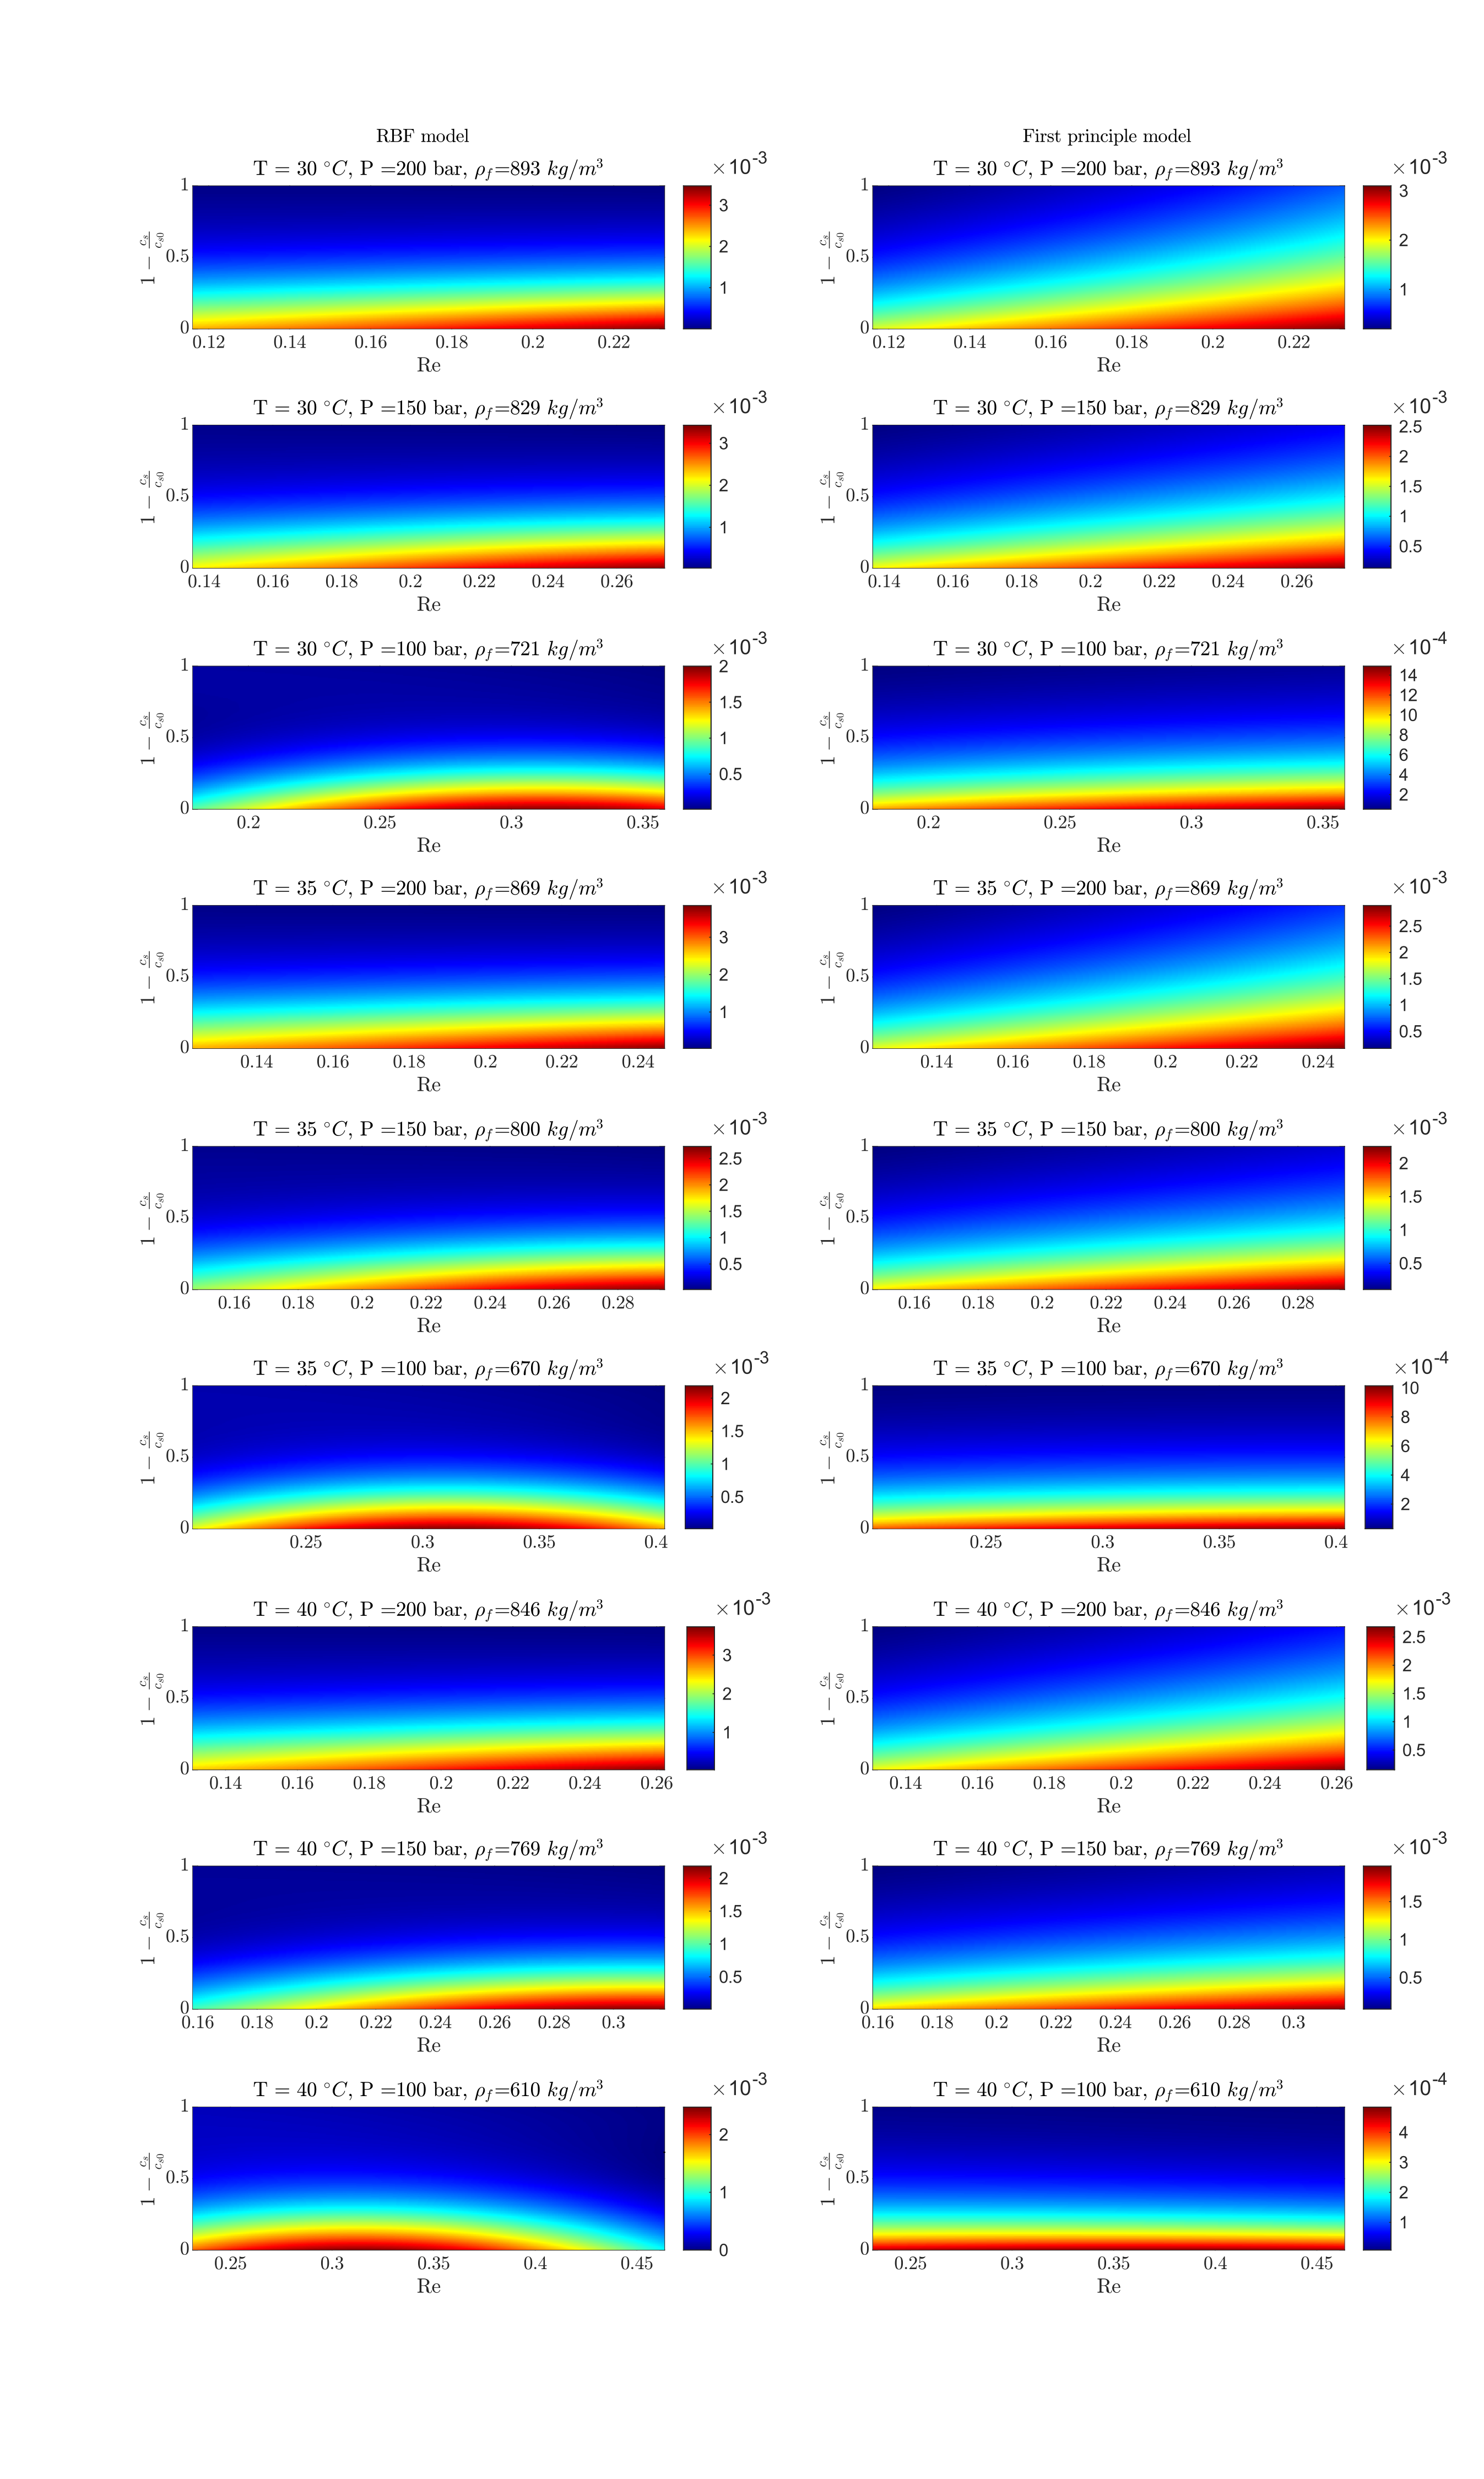
\includegraphics[trim = 1cm 2.5cm 0.5cm 1.8cm,clip,height=0.95\textheight]{/Results/RBFvsFP.png}
		\caption{Comparison of the kinetic term obtained from the first principle model and the RBF model}
		\label{fig:RBF_FP}
	\end{figure*}
	
	Good agreement between the simulation results and the dataset can be observed in Figure \ref{fig:RBF}. The figure compares the yield curves for the first principle (dashed line) and the RBF-based model (dotted line). The calculated mean square error and standard deviation as presented in Table \ref{tab:Modelling_Error}.
	
	\begin{table*}[h]
		\centering
		\adjustbox{max width=\textwidth}{%
			%\small{
				\begin{tabular}{ l|ccccccccccccc }
					\hline 
					Experiment			&1 		& 2 		& 3 	 & 4 	  & 5 	   &6 	   & 7	   & 8	   & 9	   & 10    & 11    & 12	\\  \hline
					Mean squared error of the cumulative measurement	&0.0023 & 0.0026 	& 0.0252 & 0.0316 & 0.0497 &0.0087 & 0.0205& 0.0047& 0.0028& 0.0033& 0.0060& 0.0014	\\  
					Mean squared error of the independent measurements	&0.0003 & 0.0006 	& 0.0021 & 0.0018 & 0.0012 &0.0012 & 0.0017& 0.0016& 0.0001& 0.0011& 0.0004& 0.0004	\\  
					Standard deviation of error of the independent measurements	&0.0182 & 0.0255 	& 0.0458 & 0.0426 & 0.0274 &0.0356 & 0.0396& 0.0409& 0.0094& 0.0349& 0.0208& 0.0195	\\  \hline
			\end{tabular} }
			\caption{Error between experimental data and model predictions}
			\label{tab:Modelling_Error}
		\end{table*}
	
	\begin{figure*}
		\centering
		\begin{subfigure}[b]{0.32\textwidth}
			\centering
			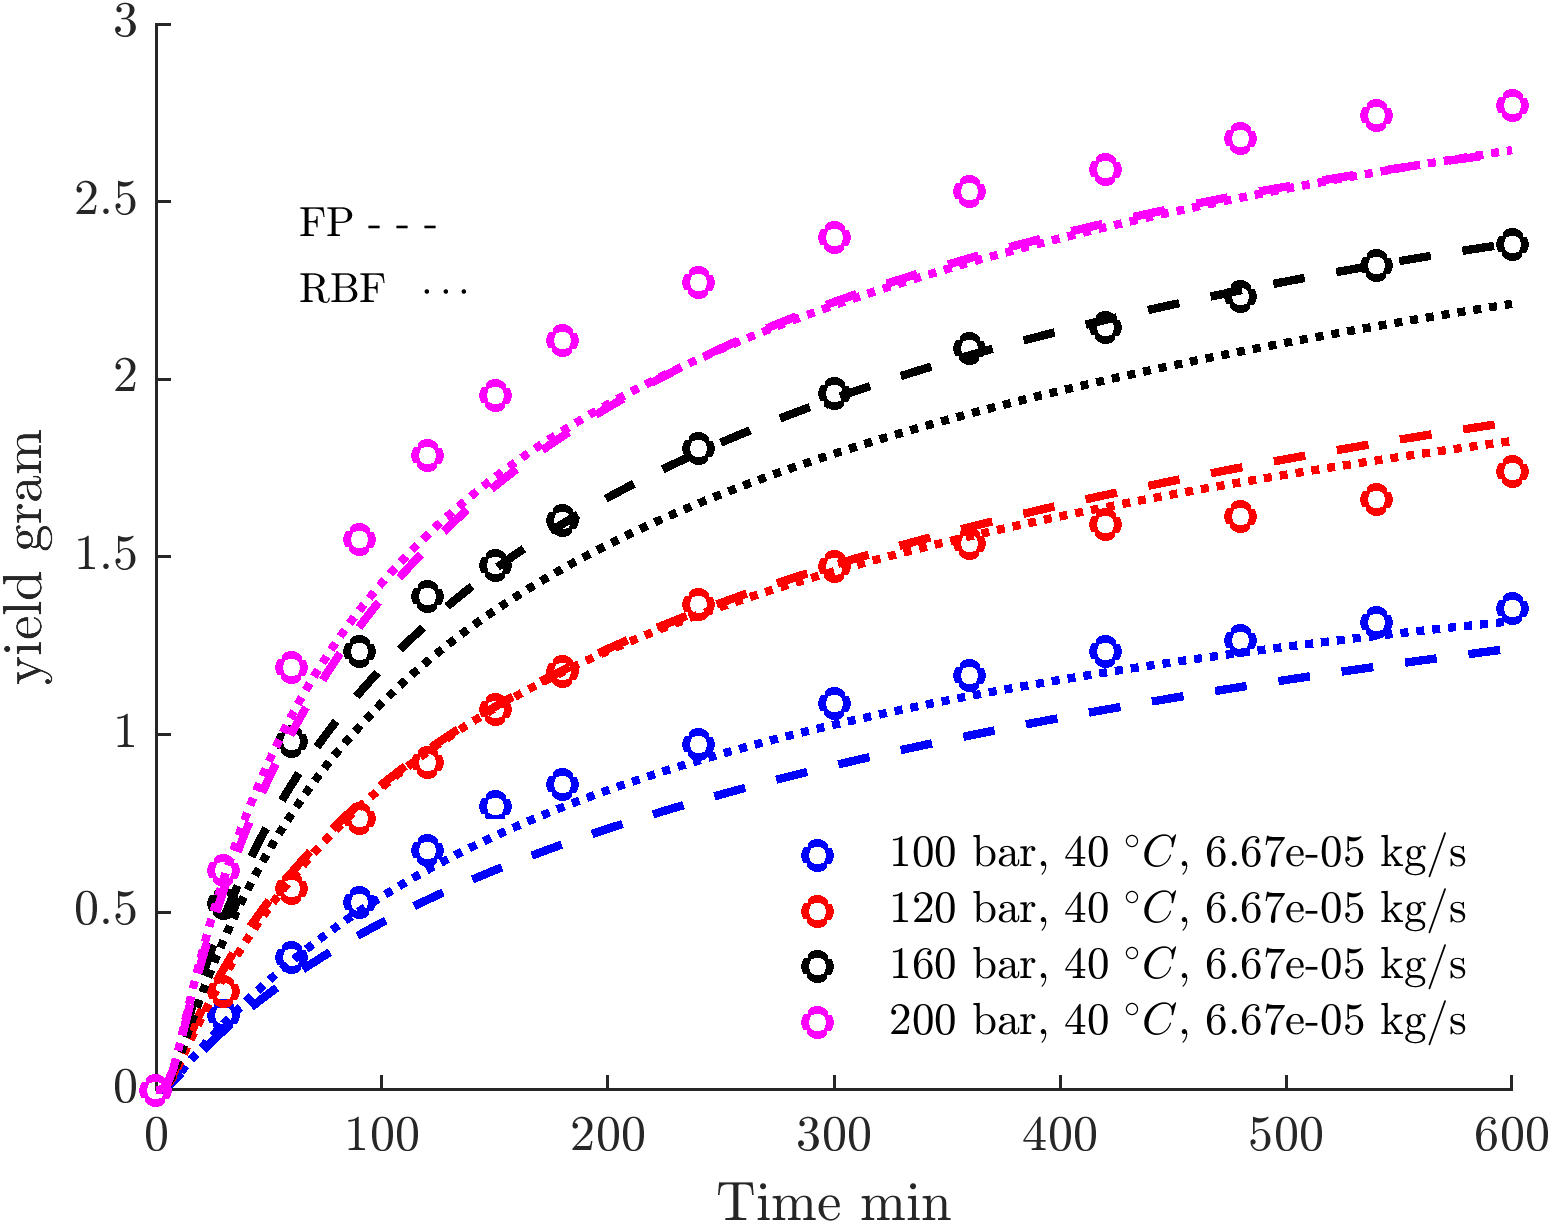
\includegraphics[width=\textwidth]{/Results/1.png}
			\caption{Simulation results}
			\label{fig:RBF_1}
		\end{subfigure}
		\hfill
		\begin{subfigure}[b]{0.32\textwidth}
			\centering
			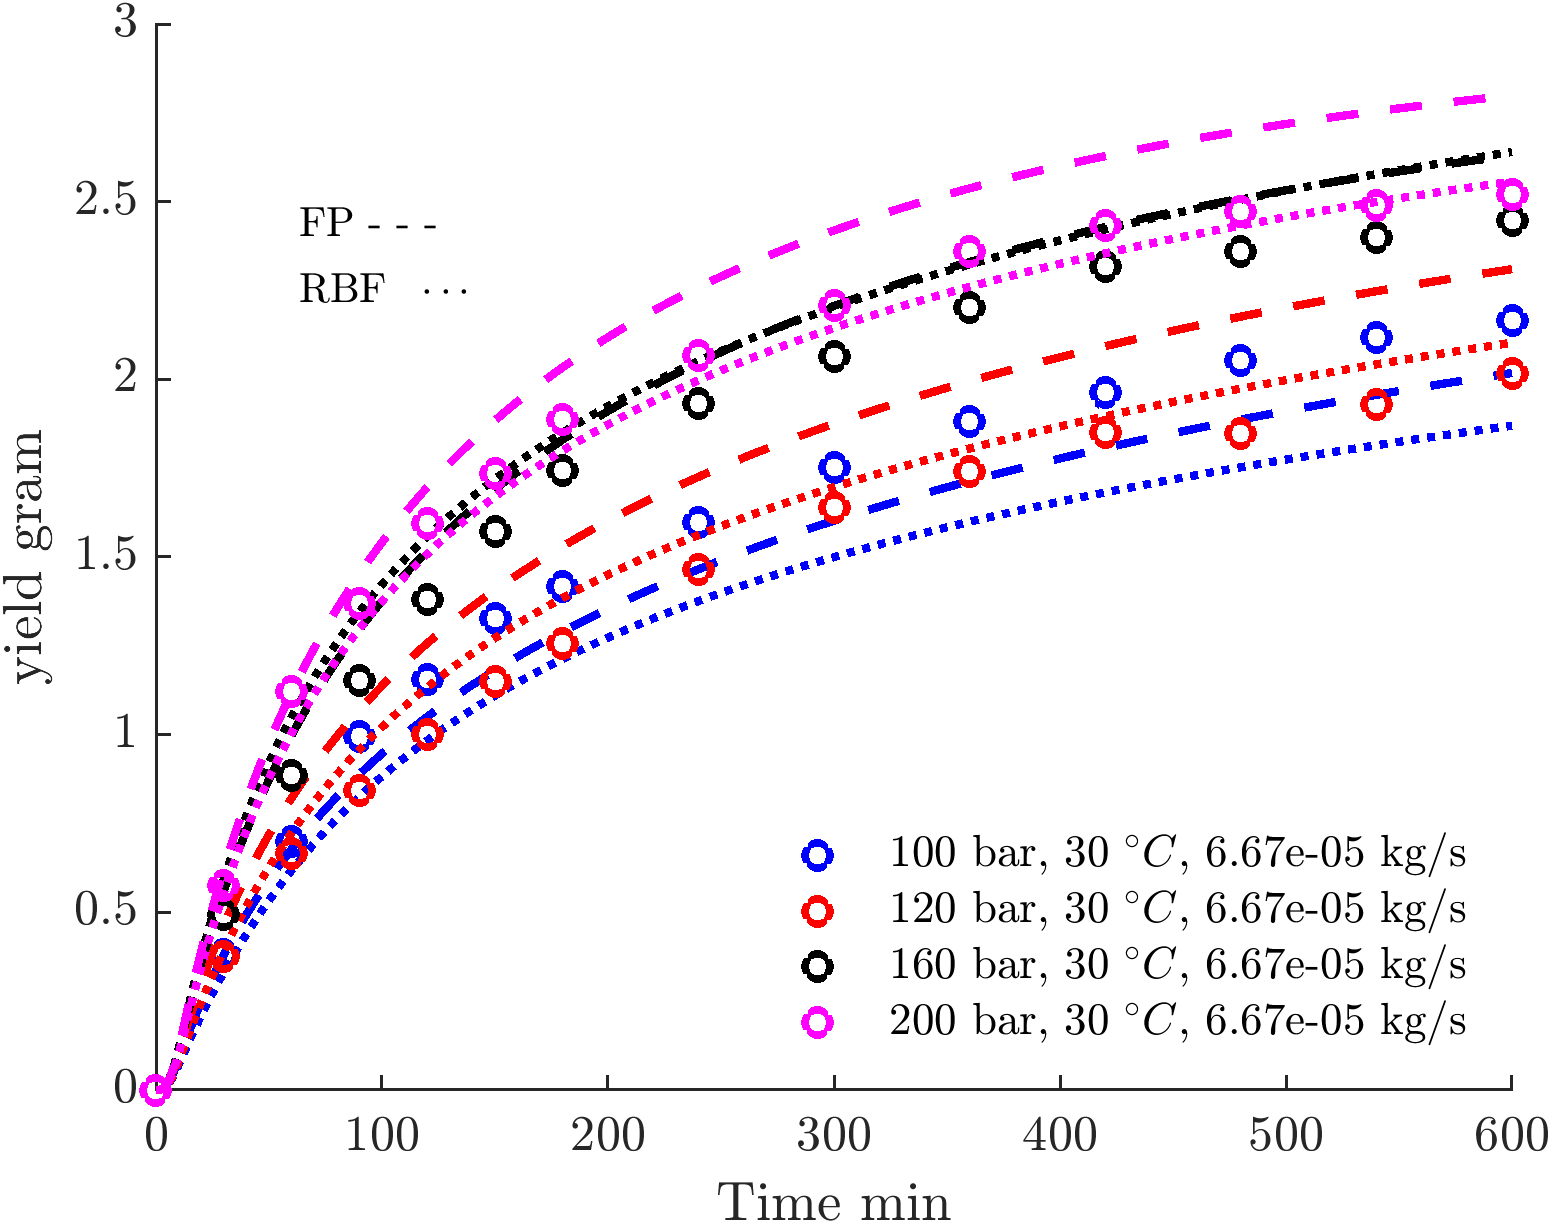
\includegraphics[width=\textwidth]{/Results/2.png}
			\caption{Simulation results}
			\label{fig:RBF_2}
		\end{subfigure}
		\hfill
		\begin{subfigure}[b]{0.32\textwidth}
			\centering
			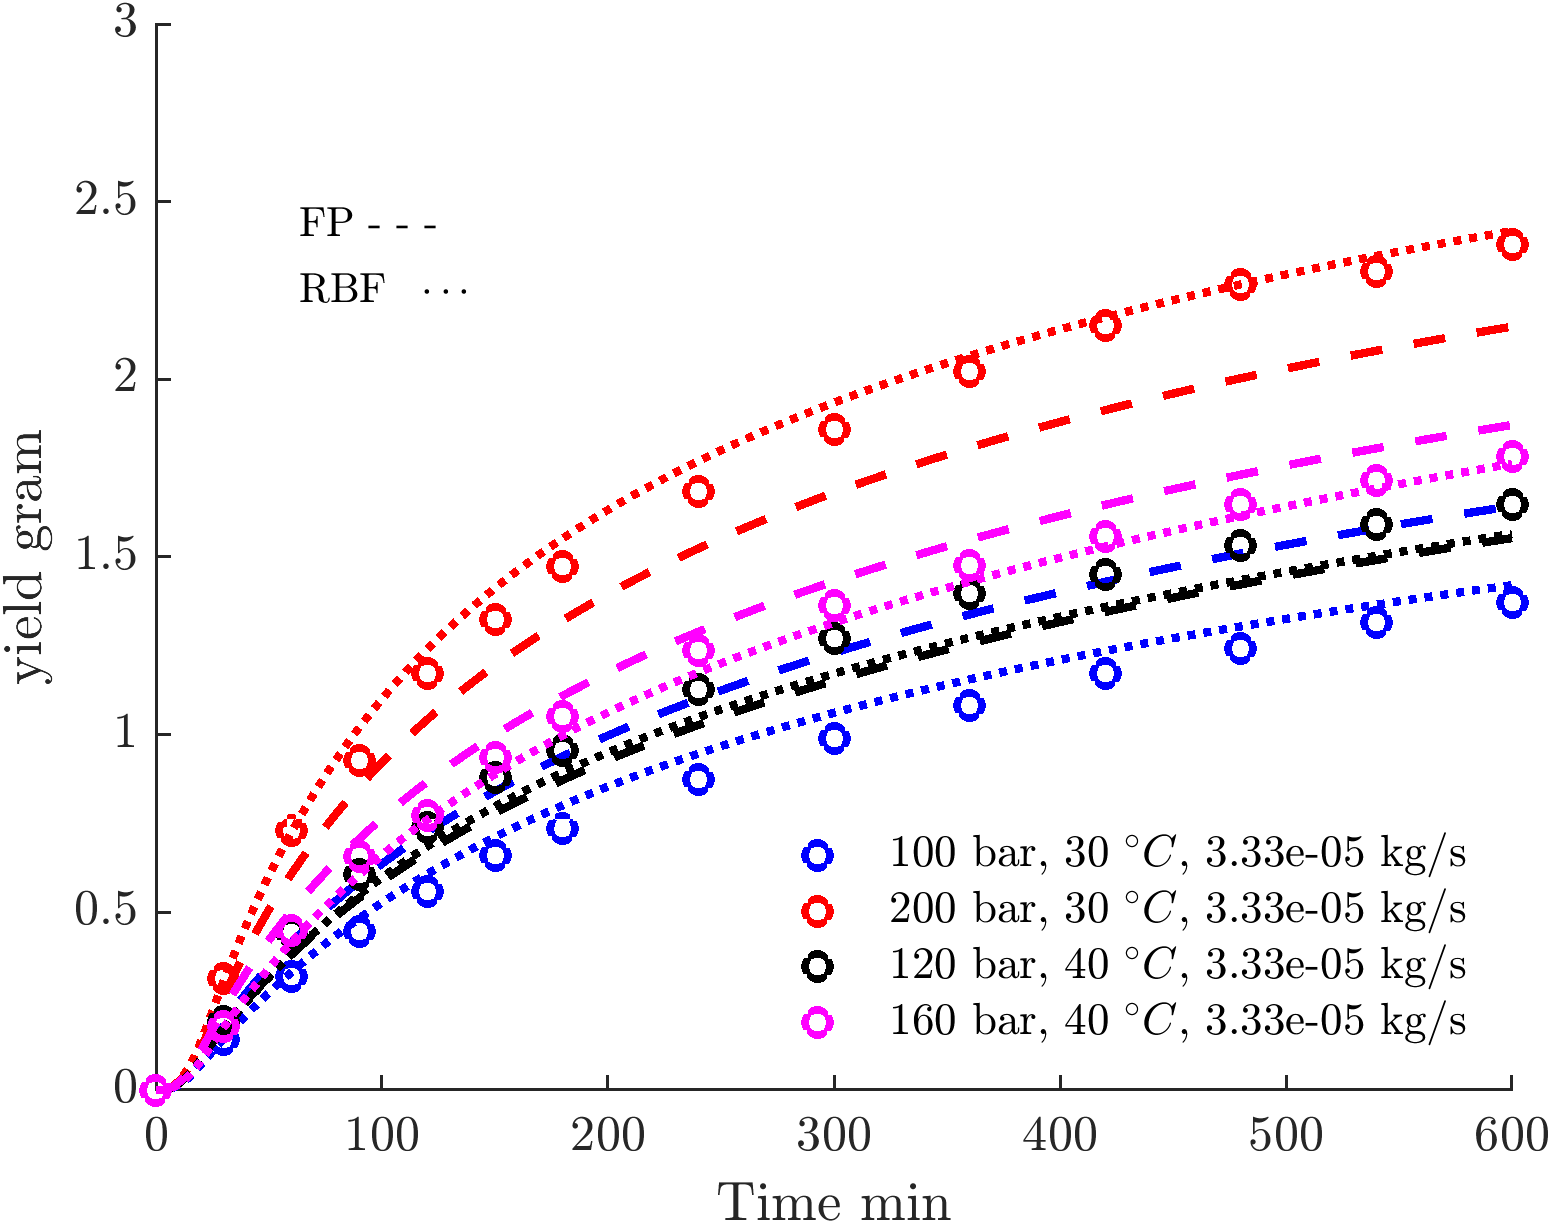
\includegraphics[width=\textwidth]{/Results/3.png}
			\caption{Simulation results}
			\label{fig:RBF_3}
		\end{subfigure}
		\caption{Comparison between the First Principle model(FP), the data-driven model (RBF) and the dataset}
		\label{fig:RBF}
	\end{figure*}
				
\end{document}